\chapter{Engraving System}
\label{chap:EngravingSystem}

This chapter describes the Mashcima engraving system we developed. We created a~custom engraving system for handwritten music to serve as an~advanced data augmentation tool. We opted to write a~new system from scratch, because of the flexibility we needed. We will talk about the specific requirements for the engraving system. We will briefly overview the inner workings of the system - how it understands the input (Mashcima encoding), what are the basic building blocks from which a~staff image is engraved, what are the most important events that happen during engraving. We will talk about the shortcomings of the system and how it could be extended in the future.


\section{Why Custom Engraving System}

In the thesis introduction (chapter \ref{chap:Introduction}) we stated that there is only a~single dataset containing handwritten staves of music. There are other handwritten music datasets, but they either contain only symbols, or they are derived from CVC-MUSCIMA. Using this dataset as-is for training is not plausible, because it contains far too few symbol combinations.

We are not the first to realize this issue. The HMR baseline article (\cite{HmrBaseline}) talks about using data augmentation and transfer learning to solve the lack of training data. They propose a~model to be trained on printed music, of which there's abundance. After that, the model is fine-tuned by training on the CVC-MUSCIMA dataset. The results they obtained are impressive, considering the method they used. To help with the process, they used data augmentation, like dilation, erosion, and blurring, and even measure shuffling.

We propose to use more sophisticated data augmentation. Specifically, we want to shuffle the data on the level of individual musical symbols. The reason we choose this approach is that we have access to the MUSCIMA++ dataset (\cite{MuscimaPP}). This dataset contains a~lot of additional information regarding the CVC-MUSCIMA dataset, which includes segmentation masks of individual symbols and their relationships. We want to use these masks to engrave entirely new staves of music.

We will also build our own engraving system because engraving handwritten music is something that existing engraving systems don't focus on. Handwritten music is very different from printed music. Symbol positions vary, notehead shapes may differ from note to note within a~single staff, slant angle may also change. We tried looking at Abjad\footnote{\href{https://github.com/Abjad/abjad}{https://github.com/Abjad/abjad}} --- a~python package for engraving music that uses Lilypond\footnote{\href{http://lilypond.org/}{http://lilypond.org/}} at its core. Lilypond can load custom fonts, but those have to be in vector form, not raster masks. Also, there's no way to introduce a~controlled variability and randomness into the engraving process. When we considered the options, we decided to create or own system, since it would be faster and we would have the ability to modify it in the future.


\section{Requirements}

We are not trying to produce PDF files as the other engraving systems do. Our goal is to produce a~single staff of handwritten music, as a~raster image. This image should look as similar as possible to a~cropped image of a~staff from the CVC-MUSCIMA dataset. This means the image is already binarized, it has comparable resolution and the image has about three times the height of the staff it contains (the height of the staff lines).

This similarity can be accomplished by using symbols from MUSCIMA++. On page 19 of writer 1, there's an~empty staff. We take the mask of the staff lines and produce an~empty image of proper dimensions containing the empty staff lines. The staff lines are almost perfectly horizontal (they wobble up and down by a~few pixels, but don't drift), therefore we will use them to create a~lookup table for converting pitch numbers to pixel offset in the $y$ axis. This will act as our blank canvas, from which we will start. \emph{Canvas} is an~actual term used in the codebase.

\begin{figure}[h]
    \centering
    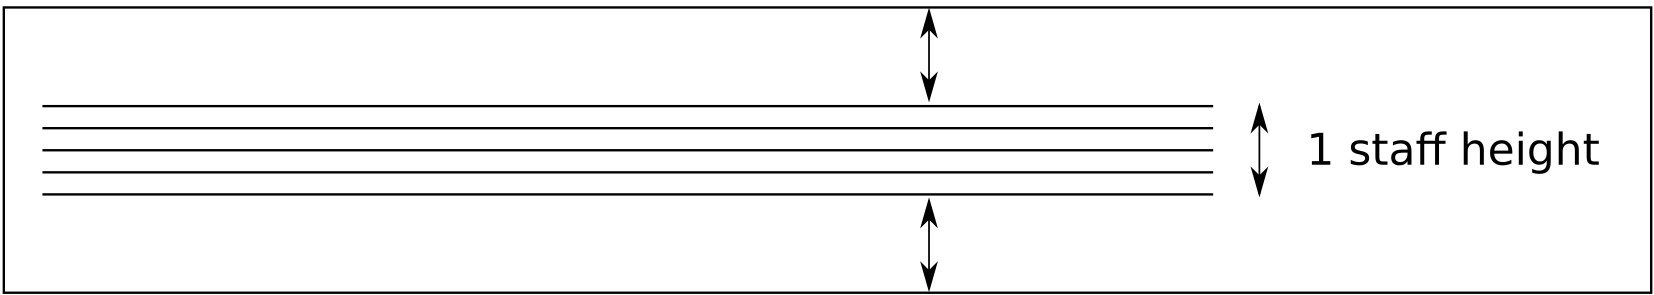
\includegraphics[width=140mm]{../img/staff-padding}
    \caption{Empty staff and the padding to the edge of the engraved image.}
    \label{fig5:EmptyStaffWithPadding}
\end{figure}

By trying to mimic the look of CVC-MUSCIMA, we will remove a~lot of problems that we would otherwise face. We don't need to perform any distortion removal, alignment, cropping, preprocessing, and binarization. All this is already performed on the source data we use. This lets us focus only on the engraving system, which is complicated enough by itself.


\section{Token Groups and Canvas Items}

The Mashcima encoding defines the concept of token groups. It is not discussed in the chapter on the encoding, because it is not so important for the encoding itself. A~\emph{token group} is a~group of tokens, that has one main token and then all the attachments of that token. So for example a~quarter note with a~sharp and a~staccato dot is represented by three tokens, but it is a~single token group. A~token group is all the tokens that belong to some non-attachment token.

Token groups are used in Mashcima annotation validation. When proper attachment ordering is checked, the annotation is first grouped into token groups and then each group has its attachment order checked. It also helps us to hide away all the attachment tokens and focus only on the important tokens.

Two special kinds of token groups are key signatures and numeric time signatures. It again makes sense to treat a~time signature as a~single object and since it's a~multitude of tokens, it's represented by a~token group.

Token groups are important because they map directly onto canvas items. A~\emph{canvas item} is something on the staff, that takes up horizontal space and can be rendered. Canvas item represents a~barline, a~note, a~rest. Attachments, like accidentals and dots, are not canvas items but are part of some given canvas item and they modify its appearance. Canvas items are placed on the staff right after each other with some randomized amount of padding between them. A~canvas item has all the vertical space it can have and it decides, where to draw itself vertically. You can see the bounding boxes of individual canvas items in figure~\ref{fig5:CanvasItems}.

\begin{figure}[h]
    \centering
    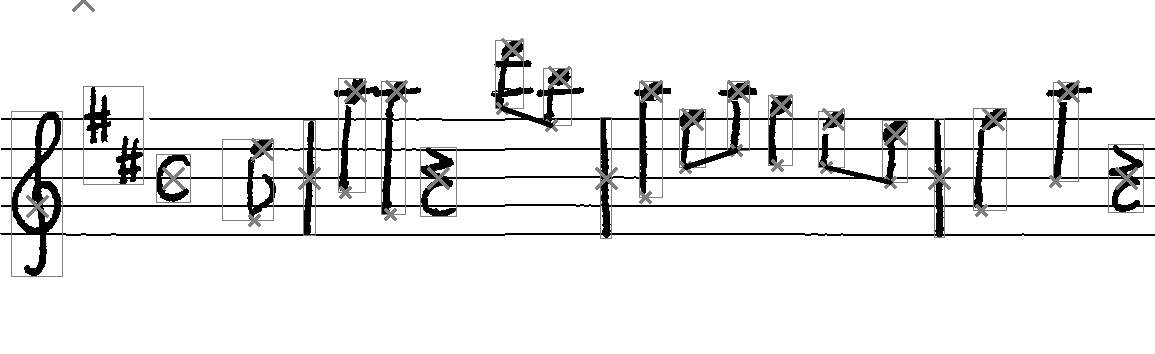
\includegraphics[width=140mm]{../img/canvas-items}
    \caption{Canvas items with bounding boxes.}
    \label{fig5:CanvasItems}
    \medskip
    \small
    A bounding box encloses all sprites of a canvas item. The large cross is the origin and it used to position the items vertically. Smaller crosses are marking where a stem ends and a beam attaches. A key signature does not use its origin point, so it's left at the top of the image.
\end{figure}


\section{Rendering Flow}

The process of converting an~annotation to an~image has a~couple of important steps:

\paragraph{Canvas instance is created} An~instance of the \verb`mashcima.`\allowbreak\verb`Canvas` class is created, so that canvas items could be added into it.

\paragraph{Canvas items are added} The annotation is grouped into token groups and those groups are mapped onto canvas items. This step just feeds the semantic information from the encoding system to the engraving system. This step is performed by the \verb`annotation_`\allowbreak\verb`to_canvas` function inside \verb`mashcima/`\allowbreak\verb`annotation_`\allowbreak\verb`to_image.py`.
\\

The following steps happen inside the \verb`Canvas`\allowbreak\verb`.render(...)` method.

\paragraph{Canvas construction is finished} This goes over the added canvas items and extracts information about slurs and beams. This step also validates that beams and slurs are properly formed. This extracted information is used later during the rendering of slurs and beams.

\paragraph{Sprites are selected} Each canvas item gets to choose specific symbol sprites (images) to use for rendering. These sprites are chosen from a~symbol sprite repository, represented by the class \verb`mashcima`\allowbreak\verb`.Mashcima` inside the file \verb`mashcima/`\allowbreak\verb`__init__.py`.

\paragraph{Sprites and canvas items are placed} With specific sprites selected, dimensions are now known and so everything can be positioned properly. Canvas items are positioned from left to right one at a~time. Each time a~canvas item is placed, it also places its internal sprites (and attachments and other ornaments) and determines its total width.

\paragraph{Beams are placed} With note positions known, we can calculate the proper position and angle for each beam. Once the beam position is calculated, the length of stems of all corresponding notes is adjusted to match the beam.

\paragraph{Everything is rendered} Canvas items, beams, and slurs are rendered. The order is not important, because the resulting image is binary.


\section{Slurs and Beams}

There are only a~few symbols that are not taken from the MUSCIMA++ dataset as images but are instead rendered manually. Those are slurs and beams. MUSCIMA++ does contain binary masks of these symbols, but the problem is that they cannot be simply moved to a~different position and rendered. They rely heavily on the position of other symbols and therefore they would need to be stretched, rotated, and skewed to render properly.

Slurs have some pre-defined attachment points they can use and the specific attachment point is chosen by the way a~note is flipped. Once the two points are chosen, the slur is rendered as a~parabola. This approach far too naive and simplified, so it doesn't capture the whole variability of a~handwritten slur. We think this is the reason the model makes so many mistakes regarding slur placement.

\begin{figure}[h]
    \centering
    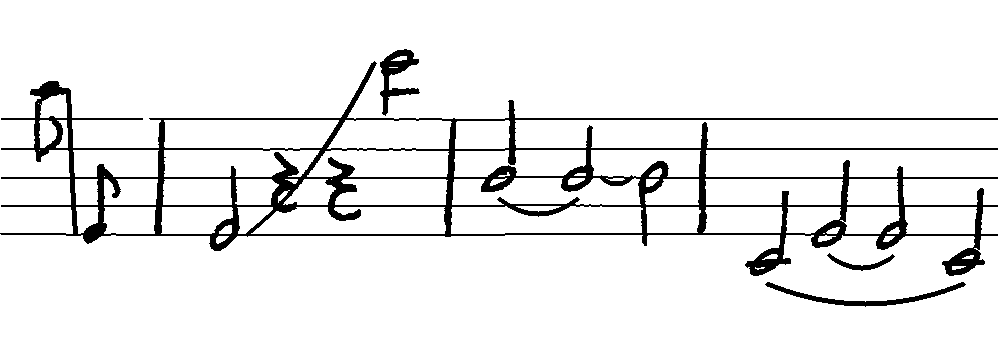
\includegraphics[width=120mm]{../img/failed-slurs}
    \verb`e6 ( ) e-4 | h-4 ( qr qr ) h8 | h0 ( ) h0 ( ) h0 |`
    \verb`h-6 ( h-4 ( ) h-4 ) h-6`
    \caption{Sometimes slur rendering doesn't look nice.}
    \label{fig5:FailedSlurs}
    \medskip
    \small
    Slurs cannot move other items around or create additional space. Slur doesn't move away when it intersects other symbols. Nested slurs are allowed, although not recommended.
\end{figure}

Beams face many similar problems as slurs. They are also rendered manually, as straight lines. This again does not capture the real world. Beams are often curved or they have a~gap between itself and a~note stem. This again seems to be the source of many mistakes, especially with the writer 49, who leaves a~lot of gaps between beams and stems.


\section{Multi-staff images}

Staves are usually so close together, that cropping a~single staff with proper space around it will usually crop parts of symbols from the staves above and below. We want to capture this property of real-world data in our synthetic data.

We can take our rendering system and run it three times to render three staves into a~single image. We crop out the middle staff we actually want. It can be used with some variations --- having staff only above, or only below.

Multi-staff rendering can be performed by the \verb`multi_`\allowbreak\verb`staff_`\allowbreak\verb`annotation_`\allowbreak\verb`to_image` function inside \verb`mashcima/`\allowbreak\verb`annotation_`\allowbreak\verb`to_image.py` file.

\begin{figure}[h]
    \centering
    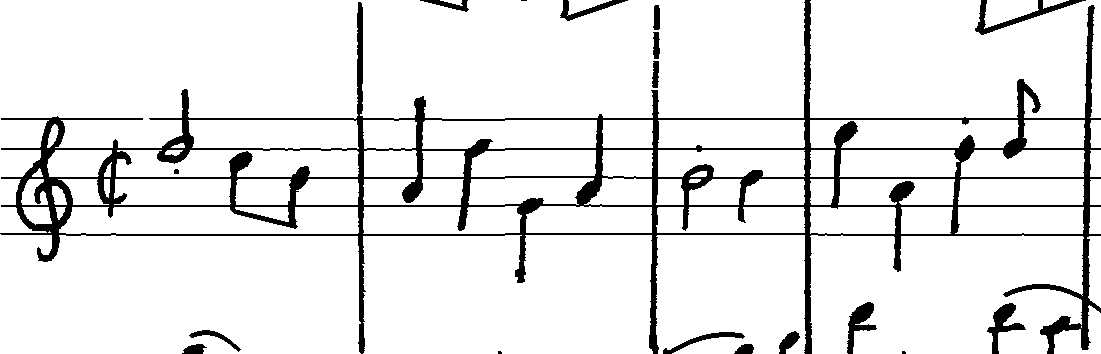
\includegraphics[width=120mm]{../img/multi-staff}
    \caption{Rendering staves above and below with long barlines.}
    \label{fig5:MultiStaff}
\end{figure}


\section{Additional Deformation and Normalization}

Affine transformation is applied to the produced image to make the model resilient to changes in image positioning, perspective, size, and rotation. This transformation is a~subtle, but very important step of the synthetic data preparation.

Finally, before the image is fed into the model, it's normalized to a~specified height, while preserving the aspect ratio. The resulting image can look like this:

\begin{figure}[h]
    \centering
    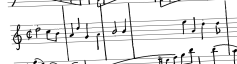
\includegraphics[width=120mm]{../img/normalized-image}
    \caption{Skewed and normalized to 64 pixels in height.}
    \label{fig5:NormalizedImage}
\end{figure}


\section{Parameters}

There are many places where the engraving system makes an arbitrary decision. This section attempts to list most of them. The list is not exhaustive. The goal is to give you an idea of how the system works.

\begin{itemize}
    \item Sprites are selected randomly from a repository of all sprites. This selection has the most impact on the variability of the resulting image. The repository contains sprites from all writer so this selection process mixes up symbols from different writers.
    \item Noteheads and stems are not mixed --- a given note sprite will always have its corresponding stem sprite when engraved.
    \item A canvas item has a pivot that is placed according to the item's pitch. This placement is not randomized (vertically) because sprite selection does a good job of it already.
    \item A note will have many sprites attached (accidentals, duration dots, staccato) and they are also chosen randomly from the sprite repository. Their position is slightly randomized. Sometimes additional rules are applied (e.g. to prevent duration dots from landing on staff lines and not being visible).
    \item Canvas items are placed from left to right with random padding inserted in between.
    \item Barlines can be short or tall. This depends on whether there are staves rendered above and below our staff.
    \item Note stem orientation depends on the note position. Lower-pitched notes point stems up and vice versa. Notes around the centerline have stem orientation randomized.
    \item A given note has three slur attachment points --- before, below, and after the notehead. When notes on both ends of a slur have stems pointing in the same direction, the below points are used. Otherwise, the before and after points are used. When below attachment points are used, slur curves with the notes. Otherwise, the curvature is randomized.
    \item Slurs are rendered as parabolas intersecting three points --- the attachment points and one midpoint. The midpoint vertical offset defines the curvature and it is proportional to the slur length.
    \item Beamed group stem orientation is determined in the same way as for a single note, only the average pitch of the group is used.
    \item The beam is selected as a line that minimizes the distance to all notes while staying on one side of all the notes. Minimal stem length is preserved.
    \item Stems in a beamed group have their height adjusted (by stretching the sprite) to end up right on the beamline.
\end{itemize}


\section{Extensibility}

Many symbols currently can be encoded, but cannot be engraved (trills, accents, fermatas). These attachment symbols could be added relatively easily, in a~similar fashion to the way staccato dots and accidentals are rendered.

The slur and beam rendering system could be improved to better mimic the real world. The concept of attachment points for slurs is a~little bit too digital. It could be made fuzzier. Also, there are certain slur placements, that the current system does not render (like slur above a~beam). This kind of extension should not require too much redesign of the system.

It would be interesting to render tuplets. They are similar to beams and slurs in many ways. Also, dynamics and hairpins are maybe even easier to add. But they cannot currently be encoded.

Adding chords is an~interesting problem, I think the current system architecture would make it quite difficult. The note canvas item would need to be entirely redesigned.
